\documentclass[12pt,a4paper,fleqn]{report}

\usepackage[top=2.5cm,bottom=2.5cm,left=3cm,right=3cm]{geometry}

% دعم العربية (XeLaTeX)
\usepackage{fontspec}

\usepackage{polyglossia}

\usepackage{tikz}
\usepackage{tikz-3dplot}

\usetikzlibrary{arrows.meta}
\usetikzlibrary{3d}


\setmainlanguage[numerals=maghrib]{arabic}
\setotherlanguage{english}

\newfontfamily\arabicfont[Script=Arabic]{Arial}

\newfontfamily\englishfont{Times New Roman}

% تنسيق
\usepackage{setspace}
\onehalfspacing

\usepackage{graphicx}
\usepackage{caption}
\usepackage{booktabs}
\usepackage{hyperref}
\usepackage{titlesec}
\usepackage{imakeidx}
\usepackage{float}
\usepackage{amsmath}


% تحميل ملفاتك
%==================== SETTINGS ====================

% دعم الألوان
\usepackage{xcolor}

% المسافات بين الأسطر
\usepackage{setspace}
\onehalfspacing

% تنسيق الفقرات
\setlength{\parindent}{0pt}
\setlength{\parskip}{6pt}

% دعم الصور
\usepackage{graphicx}
\graphicspath{{images/}}

% الجداول
\usepackage{booktabs}
\usepackage{array}

% تحسين النص
\usepackage{microtype}

% الروابط
\usepackage{hyperref}
\hypersetup{
    colorlinks=true,
    linkcolor=blue,
    filecolor=magenta,
    urlcolor=cyan,
    pdftitle={مشروع التخرج},
    pdfauthor={بهاء الياسين},
    pdfpagemode=FullScreen,
}

% ترقيم الصفحات في الأسفل
\usepackage{fancyhdr}
\pagestyle{fancy}
\fancyhf{}
\fancyfoot[C]{\thepage}

% إزالة الخط العلوي
\renewcommand{\headrulewidth}{0pt}

% دعم القوائم
\usepackage{enumitem}

% دعم الكود البرمجي (اختياري)
\usepackage{listings}

\lstset{
    basicstyle=\ttfamily\small,
    breaklines=true,
    frame=single
}
%==================== STYLES ====================

% تنسيق العناوين
\usepackage{titlesec}

% تنسيق Chapter
\titleformat{\chapter}
{\Huge\bfseries}
{\thechapter}
{1em}
{}

% تنسيق Section
\titleformat{\section}
{\Large\bfseries}
{\thesection}
{1em}
{}

% تنسيق Subsection
\titleformat{\subsection}
{\large\bfseries}
{\thesubsection}
{1em}
{}

% المسافات بين العناوين
\titlespacing*{\chapter}{0pt}{-20pt}{20pt}
\titlespacing*{\section}{0pt}{10pt}{10pt}
\titlespacing*{\subsection}{0pt}{8pt}{8pt}

% تنسيق الفهرس
\usepackage{tocloft}

\renewcommand{\cftchapfont}{\bfseries}
\renewcommand{\cftsecfont}{}
\renewcommand{\cftchappagefont}{\bfseries}

% مسافات الفهرس
\setlength{\cftbeforechapskip}{5pt}

% دعم اتجاه عربي أفضل
%\raggedleft

% تنسيق الصور
\usepackage{caption}
\captionsetup{
    justification=raggedleft,
    singlelinecheck=false
}

% تنسيق الجداول
\renewcommand{\arraystretch}{1.5}

% أوامر مساعدة
\newcommand{\HRule}{\rule{\linewidth}{0.5mm}}

% تحسين عرض الكود
\lstdefinestyle{mystyle}{
    backgroundcolor=\color{gray!10},
    commentstyle=\color{green},
    keywordstyle=\color{blue},
    numberstyle=\tiny\color{gray},
    stringstyle=\color{red},
    basicstyle=\ttfamily\small,
    breaklines=true,
    frame=single
}

\lstset{style=mystyle}

\makeindex[columns=2, title=الفهرس, options= -s resources/styles/indexstyle.ist, intoc]
\indexsetup{level=\chapter*,toclevel=chapter}

%==================== بداية المستند ====================
\begin{document}

%==================== صفحة الغلاف ====================
\makeatletter

\newcommand*{\gradeType}[1]{\gdef\@gradeType{#1}}
\newcommand*{\firstExaminer}[1]{\gdef\@firstExaminer{#1}}
\newcommand*{\secondExaminer}[1]{\gdef\@secondExaminer{#1}}
\newcommand*{\matrikelnr}[1]{\gdef\@matrikelnr{#1}}
\newcommand*{\submitDate}[1]{\gdef\@submitDate{#1}}

\renewcommand*{\maketitle}{
	\begin{titlepage}
		
		\newgeometry{left=2.5cm,right=2.5cm,top=2.0cm,bottom=2.5cm}



		\noindent
        \begin{minipage}[t]{0.35\textwidth}
            \centering
            
           
            
\includegraphics[width=0.6\linewidth]{resources/images/logo}\\[0.3cm] 
            
            
            \textbf{الجمهورية العربية السورية}\\
            \textbf{ وزارة الدفاع}\\
            
            
        \end{minipage}\hfill 
        
        
        \vspace{3cm} 



		\begin{center}
					
		
			{\Large \@title\par}
			\vskip 0.5cm
			{\large \bfseries  بحث علمي   \par}
			\vskip 0.5cm
			%{\large مقدم لنيل\\ \bfseries \@gradeType}
			%\vskip 0.5cm
			%{\large جامعة حلب}
			%\vskip 0.5cm
			%{\large  كلية الهندسة الكهربائية و الألكترونية\\ قسم هندسة التحكم الآلي والأتمتة الصناعية}
			\vfill
			\begin{minipage}{0.5\textwidth}
        		\centering
        		\large
        		\textbf{اعداد }\\[0.3cm]
        		{\Large \@author}
    			\end{minipage}
		\end{center}
		\restoregeometry
	\end{titlepage}
}
\makeatother

\title{ دراسة تحليلية  للنمذجة الرياضية وتطوير استراتيجيات التحكم لذراع روبوتية من نوع SCARA}

\author{بهاء الياسين}



\pagenumbering{alph}
\maketitle

%==================== الصفحات التمهيدية ====================
\pagenumbering{Roman}

\chapter*{الملخص}

يقدم هذا المشروع دراسة تحليلية وتطبيقية شاملة للنمذجة الرياضية وتصميم استراتيجيات التحكم المتقدمة للروبوت الصناعي ذي المفاصل الأفقية \LR{(SCARA)}.     يهدف البحث إلى تحقيق تتبع مسار دقيق وسريع يواكب التغيرات التشغيلية والاضطرابات الخارجية.

يبدأ المشروع بدراسة النمذجة الحركية \LR{(Kinematic Modeling)} للروبوت، حيث تم استنتاج معادلات الحركة المباشرة \LR{(Forward Kinematics)} لتحديد موضع وتوجيه المؤثر النهائي في الفراغ التشغيلي بناءً على إحداثيات المفاصل. وفي الجانب التحليلي الأعمق، تم اشتقاق النموذج الديناميكي بدقة عالية باستخدام معادلات لاغرانج-أويلر، حيث يتميز هذا العمل بإدراج تغير كتلة الحمل \LR{$m_L$} بشكل صريح ومباشر كمتغير أساسي مدمج داخل بنية النموذج ومُقَدِّر الديناميكا اللحظي. هذا الإدراج المباشر مكَّن المنظومة من تحديث حسابات مصفوفة العطالة وشعاع الجاذبية آنياً بناءً على القيمة اللحظية للحمل، مما يضمن محاكاة فيزيائية دقيقة تواكب الحمولات الحقيقية للروبوت.

وبناءً على هذا النموذج الرياضي المطور، تم تصميم ومحاكاة ثلاث استراتيجيات تحكم رئيسية وتقييم أدائها؛ حيث طُبِّق متحكم تناسبي-تكاملي-تفاضلي \LR{(PID)} كمعيار مرجعي لبيان عيوب تراكم الأخطاء وتأثير الجاذبية، تلاه تصميم متحكم بالانزلاق \LR{(SMC)} لتوجيه الذراع بنعومة وفصل ديناميكا المحاور. ولتوفير أقصى درجات المتانة ضد أخطاء النمذجة المتبقية أو الاحتكاك غير المنمذج، تم تطوير متحكم عزم محسوب تكيفي متقدم يعتمد على مصفوفة الانحدار \LR{(Regressor-Based ACTC)}، مدعوماً بقانون تحديث يشتمل على عامل التسريب \LR{)$\sigma$-modification)} لضمان استقرار المعاملات المقدرة ومنع انجرافها رياضياً.

تمت محاكاة النظام بالكامل في بيئة \LR{MATLAB/Simulink}، حيث أثبتت النتائج التطبيقية كفاءة استراتيجيات التحكم المعتمدة على النموذج \LR{(Model-Based)} وقدرتها الفائقة على تحقيق استجابة ديناميكية ناعمة ومستقرة تماماً بدون تجاوز \LR{(Overshoot)}، مع تصفير خطأ الحالة المستقرة للمفصل الانسحابي والمفاصل الدورانية تحت مختلف ظروف التشغيل والحمولات المتغيرة. \clearpage % ملخص المشروع


%==================== الفهرس ====================
\tableofcontents
\clearpage

%==================== المحتوى ====================
\pagenumbering{arabic}

\chapter{المقدمة }
\label{ch:introduction}

تعتبر المناورات الروبوتية، وعلى وجه الخصوص الروبوتات ذات المفاصل الأفقية (\LR{SCARA})، أنظمة ديناميكية شديدة اللاخطية ومتعددة المداخل والمخارج (\LR{MIMO}). إن تحقيق أداء حركي عالي الدقة في هذه الأنظمة لا يقتصر فقط على التصميم الميكانيكي، بل يعتمد بشكل جوهري على عمق الفهم الرياضي للتداخلات الحركية (\LR{Dynamic Coupling})، وقوى القصور الذاتي، وتأثيرات كوريوليس والجاذبية. ومع تزايد متطلبات التطبيقات الحديثة للتعامل مع مسارات معقدة وحمولات متغيرة ($m_L$)، تصبح الحاجة إلى استراتيجيات تحكم متقدمة قادرة على ترويض هذه الديناميكا أمراً حتمياً لا يمكن تجاوزه.

تقليدياً، يتم اللجوء إلى تقنيات التحكم الخطي المستقل لكل مفصل، مثل المتحكمات التناسبية-التكاملية-التفاضلية (\LR{PID}). ورغم بساطتها، إلا أن أداءها يتدهور بشدة عند السرعات العالية بسبب التجاهل التام للتداخلات الديناميكية بين المفاصل. وفي المقابل، تقدم خوارزميات التحكم المعتمدة على النموذج، مثل التحكم بالعزم المحسوب (\LR{CTC})، حلاً رياضياً مثالياً من خلال مبدأ الاستخطاط بالتغذية العكسية (\LR{Feedback Linearization}) لإلغاء اللاخطية تماماً. لكن هذا الإلغاء الجبري يتطلب تطابقاً تاماً بين النموذج الرياضي المحسوب والنظام الفيزيائي الحقيقي، وهو افتراض يصعب تحقيقه في الواقع العملي في ظل وجود شكوك معلمية (\LR{Parametric Uncertainties}) كاحتمالية تغير كتلة الحمل المرفوع، أو وجود قوى احتكاك غير منمذجة بدقة.

لمواجهة تحديات عدم اليقين في النمذجة الرياضية، برزت نظريات التحكم المتين والتكيفي كأقوى الحلول الهندسية في نظرية التحكم الحديثة. يوفر التحكم بالانزلاق (\LR{SMC}) مناعة عالية ضد الاضطرابات، خاصة عند تعزيزه بقوانين وصول متقدمة (\LR{Proportional Rate Reaching Law}) تخفف من ظاهرة الاهتزاز (\LR{Chattering}) وتضمن وصولاً أسياً سريعاً لسطح الانزلاق. من جهة أخرى، يمثل التحكم التكيفي المعتمد على مصفوفة الانحدار (\LR{Regressor-Based ACTC}) ذروة التطور في هذا المجال؛ حيث يمنح الروبوت قدرة ذاتية على "التعلم" وتحديث معاملاته الديناميكية المجهولة لحظياً لتعويض أي تغير في الحمل. ولضمان عدم خروج هذه المعاملات عن السيطرة بسبب ضجيج الحساسات، يتم تحصين خوارزميات التحديث رياضياً باستخدام تقنيات متقدمة مثل عامل التسريب (\LR{$\sigma$-modification}).

يندرج هذا المشروع في صميم هذا التحدي الهندسي؛ حيث لا يكتفي بتطبيق خوارزميات تحكم كصناديق مغلقة، بل يغوص في البنية الرياضية العميقة للروبوت. من خلال تأسيس نموذج ديناميكي دقيق باستخدام صياغة لاغرانج-أويلر، وبناء مصفوفات العطالة والانحدار وتضمين كتلة الحمل بداخلها، ينتقل المشروع تدريجياً لترويض هذه المعادلات برمجياً وتطبيق استراتيجيات تحكم لاخطية وتكيفية متطورة. إن الهدف الجوهري من هذا البحث هو إثبات القدرة على تصميم نظام تحكم متكامل يضمن استقرار ليابونوف (\LR{Lyapunov Stability})، ويحقق تتبعاً مسارياً دقيقاً، ويتكيف بمرونة مع أعقد المتغيرات الفيزيائية، مما يشكل جسراً حقيقياً بين النظرية الرياضية البحتة والتطبيق الصناعي الموثوق.
\chapter{النمذجة الحركية (\LR{Kinematic Modeling})}
\label{ch:kinematics}

يعتبر النموذج الحركي الخطوة الأولى والأساسية في تحليل أي مناور روبوتي. يهتم هذا الفصل بدراسة حركة الروبوت من منظور هندسي صرف دون التطرق إلى القوى أو العزوم المسببة لهذه الحركة. من خلال الاعتماد على المعطيات الهندسية لأطوال الوصلات وحدود حركة المفاصل، سيتم بناء النموذج الحركي المباشر الذي يربط بين إحداثيات المفاصل الداخلية للروبوت والموضع الفراغي الديكارتي للمؤثر النهائي، وهو ما يعتبر ضرورياً لمعرفة النطاق التشغيلي للذراع وتقييم مساراتها الفراغية لاحقاً.


\section{تعيين المحاور الإحداثية (\LR{Coordinate Frames Assignment})}
\label{sec:frames}

الخطوة الأولى في خوارزمية دينافيت-هارتنبيرغ (\LR{DH}) هي ربط جملة إحداثيات ديكارتية محلية بكل وصلة من وصلات الروبوت، بدءاً من القاعدة الثابتة (\LR{Base}) وصولاً إلى المؤثر النهائي. بالنسبة للروبوت (\LR{SCARA}) المدروس، تم توجيه المحاور وفق القواعد الهندسية التالية:

 \begin{figure}[H]
     \centering
     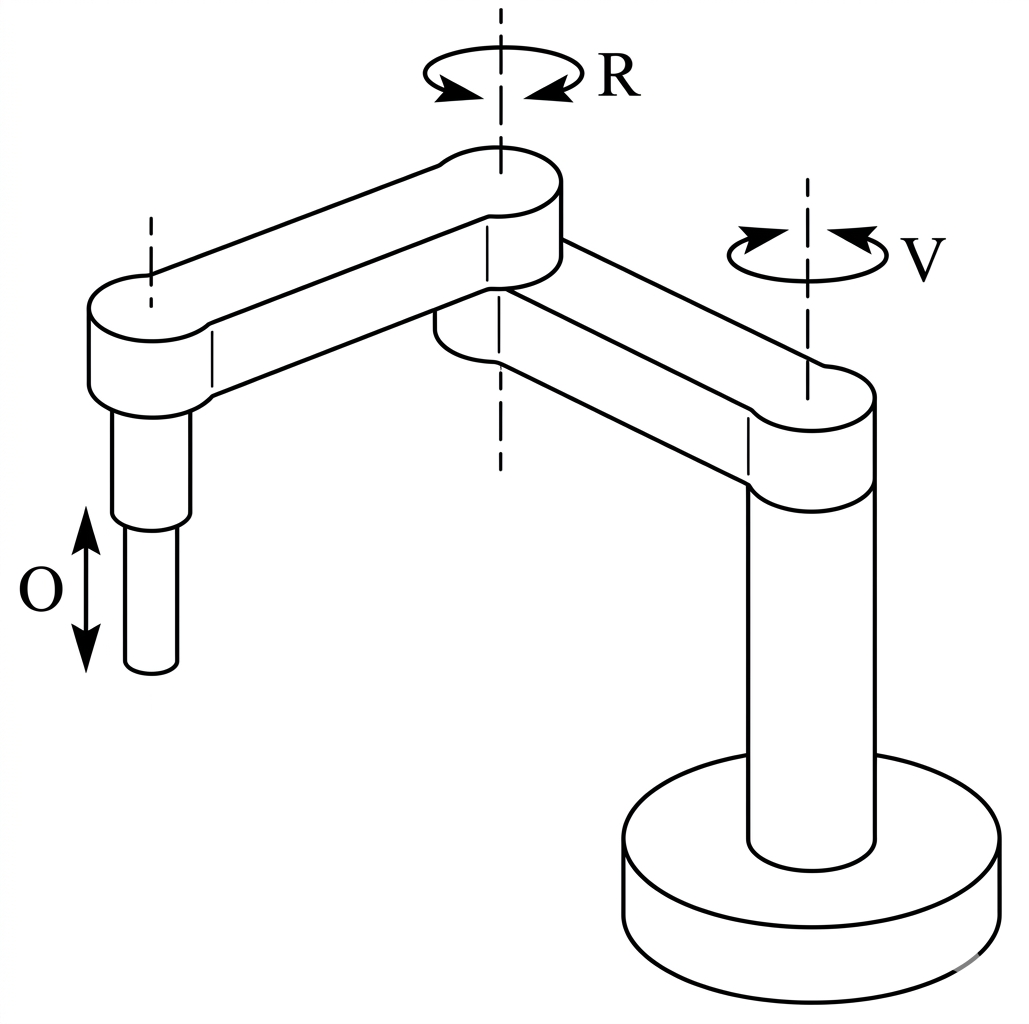
\includegraphics[width=0.7\textwidth]{resources/images/scara_arm}
%     \caption{توزيع المحاور الإحداثية على مفاصل الروبوت وفق خوارزمية \LR{DH}}
     \label{fig:frames}
 \end{figure}

\begin{itemize}
    \item \textbf{المحاور $Z_0$ و $Z_1$:} تم توجيهها عمودياً على المستوي الأفقي لتمثل محاور الدوران للمفصلين الأول والثاني.
    \item \textbf{المحور $Z_2$:} يمثل محور الحركة الانسحابية للمفصل الثالث، وتم توجيهه نحو الأسفل (باتجاه منطقة العمل).
    \item \textbf{المحاور $X_i$:} تم توجيهها على امتداد الوصلات الميكانيكية (\LR{Links}) بحيث تكون عمودية على المحور $Z_{i-1}$ وتتقاطع معه.
\end{itemize}


\section{  \LR{DH table}}
\label{sec:dh_table}

بناءً على التوزيع الهندسي لجمل الإحداثيات الموضحة في القسم السابق، يتم استخراج المعاملات الأربعة الخاصة بخوارزمية (\LR{DH}) لربط كل جملتين متتاليتين ($i-1$) و ($i$). تُعرّف هذه المعاملات الأربعة كما يلي:
\begin{itemize}
    \item $a_i$: الإزاحة الخطية على طول المحور $X_i$ من المحور $Z_{i-1}$ إلى المحور $Z_i$.
    \item $\alpha_i$: الإزاحة الزاوية (الفتل) حول المحور $X_i$ من المحور $Z_{i-1}$ إلى المحور $Z_i$.
    \item $d_i$: الإزاحة الخطية على طول المحور $Z_{i-1}$ من المحور $X_{i-1}$ إلى المحور $X_i$.
    \item $\theta_i$: الإزاحة الزاوية حول المحور $Z_{i-1}$ من المحور $X_{i-1}$ إلى المحور $X_i$.
\end{itemize}

بتطبيق هذه القواعد على البنية الميكانيكية للروبوت المدروس (\LR{SCARA})، تم استنتاج الوسطاء الحركية للمفاصل الثلاثة كما هو موضح في الجدول (\ref{tab:dh_parameters}). 

\begin{table}[H]
    \centering
    %\caption{DH table}
    \label{tab:dh_parameters}
    \renewcommand{\arraystretch}{1.5}
    \begin{tabular}{|c|c|c|c|c|c|}
        \hline
        \textbf{المفصل ($i$)} & \textbf{نوع المفصل} & \textbf{$\theta_i$} & \textbf{$d_i$} & \textbf{$a_i$} & \textbf{$\alpha_i$} \\
        \hline
        1 & دوراني (\LR{Revolute}) & $\theta_1$ & $0$ & $L1$ & $0$ \\
        \hline
        2 & دوراني (\LR{Revolute}) & $\theta_2$ & $0$ & $L_2$ & $180^\circ$ \\
        \hline
        3 & انسحابي (\LR{Prismatic}) & $0$ & $d_3$ & $0$ & $0$ \\
        \hline
    \end{tabular}
  
 
\end{table}


\section{\LR{Homogeneous Transformation Matrices}}

\label{sec:transformation}

تمثل مصفوفة التحويل المتجانس أداة رياضية قوية تدمج بين الدوران (\LR{Rotation}) والانسحاب (\LR{Translation}) في مصفوفة واحدة بأبعاد $4 \times 4$. تُعطى المصفوفة العامة للتحويل المتجانس \LR{$A_i^{i-1}$}، التي تنقل الإحداثيات من الجملة \LR{($i$)} إلى الجملة \LR{($i-1$)} وفق خوارزمية (\LR{DH})، بالعلاقة الرياضية التالية:

\begin{equation}
A_i^{i-1} = 
\begin{bmatrix}
\cos\theta_i & -\sin\theta_i \cos\alpha_i & \sin\theta_i \sin\alpha_i & a_i \cos\theta_i \\
\sin\theta_i & \cos\theta_i \cos\alpha_i & -\cos\theta_i \sin\alpha_i & a_i \sin\theta_i \\
0 & \sin\alpha_i & \cos\alpha_i & d_i \\
0 & 0 & 0 & 1
\end{bmatrix}
\label{eq:general_dh}
\end{equation}

لإيجاد مصفوفات التحويل الخاصة بمفاصل الروبوت المدروس، نقوم بتعويض المعطيات المستخرجة في الجدول (\ref{tab:dh_parameters}) داخل المعادلة العامة (\ref{eq:general_dh}). ولتبسيط الكتابة الرياضية، تم اعتماد الاختصارات المثلثية المعيارية حيث \LR{$c_i = \cos\theta_i$} و \LR{$s_i = \sin\theta_i$}.

\textbf{1. التحويل من الجملة \{1\} إلى الجملة \{0\}:}
بتعويض بارامترات المفصل الأول، حيث \LR{$d_1 = 0$}، و \LR{$a_1 = L_1$}، و \LR{$\alpha_1 = 0$}، وبما أن \LR{$\cos(0) = 1$} و \LR{$\sin(0) = 0$}، نجد:

\begin{equation}
A_1^0 = 
\begin{bmatrix}
c_1 & -s_1 & 0 & L_1 c_1 \\
s_1 & c_1 & 0 & L_1 s_1 \\
0 & 0 & 1 & 0 \\
0 & 0 & 0 & 1
\end{bmatrix}
\label{eq:A10}
\end{equation}

\textbf{2. التحويل من الجملة \{2\} إلى الجملة \{1\}:}
بتعويض بارامترات المفصل الثاني، حيث \LR{$d_2 = 0$}، و \LR{$a_2 = L_2$}، و \LR{$\alpha_2 = 180^\circ$}، وبما أن \LR{$\cos(180^\circ) = -1$} و \LR{$\sin(180^\circ) = 0$}، تتغير إشارات بعض العناصر لنحصل على:

\begin{equation}
A_2^1 = 
\begin{bmatrix}
c_2 & s_2 & 0 & L_2 c_2 \\
s_2 & -c_2 & 0 & L_2 s_2 \\
0 & 0 & -1 & 0 \\
0 & 0 & 0 & 1
\end{bmatrix}
\label{eq:A21}
\end{equation}

\textbf{3. التحويل من الجملة \{3\} إلى الجملة \{2\}:}
بتعويض بارامترات المفصل الانسحابي الثالث، حيث \LR{$\theta_3 = 0$}، و \LR{$a_3 = 0$}، و \LR{$\alpha_3 = 0$}، تنتج لدينا مصفوفة تمثل انسحاباً خطياً نقياً على المحور \LR{$Z$}:

\begin{equation}
A_3^2 = 
\begin{bmatrix}
1 & 0 & 0 & 0 \\
0 & 1 & 0 & 0 \\
0 & 0 & 1 & d_3 \\
0 & 0 & 0 & 1
\end{bmatrix}
\label{eq:A32}
\end{equation}
\section{معادلات الموضع الديكارتي (\LR{Cartesian Position Equations})}
\label{sec:position}

للحصول على التحويل الفراغي الكلي من قاعدة الروبوت إلى نقطة المؤثر النهائي، يتم ضرب مصفوفات التحويل المتسلسلة التي تم حسابها في القسم السابق ببعضها البعض:

\begin{equation}
T_3^0 = A_1^0 \cdot A_2^1 \cdot A_3^2
\end{equation}

وبعد إتمام عمليات الضرب المصفوفي وتطبيق متطابقات المجموع للزوايا المثلثية، تم التوصل إلى مصفوفة التحويل الكلية \LR{$T_3^0$}. ولتبسيط عرض المصفوفة، تم استخدام الاختصارات \LR{$c_{12} = \cos(\theta_1 + \theta_2)$} و \LR{$s_{12} = \sin(\theta_1 + \theta_2)$}:

\begin{equation}
T_3^0 = 
\begin{bmatrix}
c_{12} & s_{12} & 0 & L_1 c_1 + L_2 c_{12} \\
s_{12} & -c_{12} & 0 & L_1 s_1 + L_2 s_{12} \\
0 & 0 & -1 & -d_3 \\
0 & 0 & 0 & 1
\end{bmatrix}
\end{equation}

يمثل العمود الرابع من هذه المصفوفة شعاع الموضع الديكارتي للمؤثر النهائي في الفضاء التشغيلي. ومنه، يمكن استخلاص معادلات الحركة المباشرة النهائية \LR{($x, y, z$)} بدلالة الإحداثيات المفصلية \LR{($\theta_1, \theta_2, d_3$)} وأطوال الوصلات \LR{($L_1, L_2$)} كما يلي:

\begin{equation}
\begin{cases}
x = L_1 \cos(\theta_1) + L_2 \cos(\theta_1 + \theta_2) \\
y = L_1 \sin(\theta_1) + L_2 \sin(\theta_1 + \theta_2) \\
z = -d_3
\end{cases}
\label{eq:fk_position}
\end{equation}
يُلاحظ من المعادلة الأخيرة أن الإحداثي $(z)$ يأخذ قيمة سالبة $(-d_3)$، وهذا يتوافق رياضياً وفيزيائياً مع البنية الميكانيكية، حيث أن المحور $Z_2$ موجه نحو الأسفل، وبالتالي فإن الإزاحة الموجبة للمفصل الانسحابي ستؤدي إلى نزول الذراع أسفل مستوي القاعدة المرجعية.
\chapter{النمذجة الديناميكية (\LR{Dynamic Modeling})}
\label{ch:dynamics}

بعد استنتاج النموذج الحركي في الفصل السابق والذي يصف الحركة هندسياً، ينتقل التحليل في هذا الفصل إلى المستوى الديناميكي؛ حيث تتم دراسة القوى والعزوم المسببة لهذه الحركة. تعتبر النمذجة الديناميكية الدقيقة حجر الأساس في هندسة التحكم الآلي المتقدم، وبدونها لا يمكن تصميم خوارزميات تحكم قوية تعتمد على النموذج (\LR{Model-Based Control}) لمواجهة التداخلات الديناميكية وتغيرات الحمل.

سيتم في هذا الفصل اشتقاق النموذج الديناميكي للروبوت (\LR{SCARA}) بالاعتماد على صياغة لاغرانج-أويلر (\LR{Euler-Lagrange}). ولضمان دقة فيزيائية عالية، سيتم أخذ تغيرات الحمل بعين الاعتبار، بالإضافة إلى دمج ديناميكية المحركات الكهربائية للحصول على نموذج متكامل يمثل النظام الفعلي بدقة.


\section{النهج المعتمد للنمذجة الديناميكية والفرضيات الأساسية}
\label{sec:dynamic_approach}

يعتبر بناء نموذج ديناميكي دقيق تحدياً رياضياً، حيث تتشابك المعادلات بشكل كبير مع زيادة درجات الحرية. لتبسيط الحسابات الرياضية وتخفيف العبء الحسابي على وحدة التحكم دون الإخلال بالتمثيل الفيزيائي الدقيق للنظام، تم الاستناد إلى مجموعة من الفرضيات الهندسية والفيزيائية عند بناء النموذج الديناميكي لروبوت (\LR{SCARA}) المدروس:

\begin{enumerate}
    \item \textbf{تغير كتلة الوصلة الثالثة (تأثير الحمل):}
    بما أن المهمة الأساسية للروبوت هي نقل الحمولات (\LR{Pick and Place})، فإن الكتلة الفعالة للوصلة الثالثة لا تبقى ثابتة. لذلك، تم دمج كتلة الحمل $(m_L)$ بشكل صريح مع كتلة الوصلة الثالثة الأساسية $(m_3)$ لتشكيل كتلة مركبة جديدة متغيرة تعطى بالعلاقة $(m_3^* = m_3 + m_L)$. هذا الدمج يتطلب إعادة حساب شعاع مركز الثقل $(r_{p3})$ ومصفوفة القصور الذاتي للوصلة الثالثة في كل لحظة يتغير فيها الحمل.
    
    \item \textbf{المرجعية الصفرية للجاذبية الأرضية:}
    تم اعتبار الجملة الإحداثية المرتبطة بالمفصل الأول  هي الجملة المرجعية (\LR{Reference Frame}) لحسابات الطاقة الكامنة. وبناءً عليه، فإن شعاع الجاذبية الأرضية يؤثر عمودياً نحو الأسفل وبشكل موازٍ للمحور $Z_0$، ويُعطى بالصيغة الشعاعية $g = [0, 0, -g]^T$.
    
    \item \textbf{إهمال قوى كوريوليس والقوى النابذة:}
    في العديد من التطبيقات الصناعية لروبوتات (\LR{SCARA})، وبناءً على مسارات التشغيل التي لا تتطلب سرعات زاوية عالية، يمكن افتراض أن النظام يعمل ضمن سرعات حركية منخفضة إلى متوسطة. يتيح هذا الافتراض إهمال مصفوفة قوى كوريوليس والطرد المركزي $C(q, \dot{q})$ من النموذج الديناميكي العام، مما يبسط النموذج بشكل كبير.
\end{enumerate}

بناءً على صياغة لاغرانج-أويلر والفرضيات المذكورة أعلاه، يتبسط النموذج الديناميكي العام للروبوت (المجرد من المحركات) من شكله القياسي المعقد إلى الصيغة المصفوفية المخفضة التالية:

\begin{equation}
M(q)\ddot{q} + G(q) = \tau_{robot}
\label{eq:simplified_dynamic_model}
\end{equation}

حيث:
\begin{itemize}
    \item $M(q)$: مصفوفة العطالة أو القصور الذاتي للنظام بأبعاد $3 \times 3$.
    \item $G(q)$: شعاع قوى الجاذبية الأرضية بأبعاد $3 \times 1$.
    \item $\ddot{q}$: شعاع التسارعات المفصلية بأبعاد $3 \times 1$.
    \item $\tau_{robot}$: شعاع العزوم والقوى المحركة الفعالة عند المفاصل بأبعاد $3 \times 1$.
\end{itemize}

في الأقسام التالية، سيتم تفصيل الخطوات الرياضية لحساب مصفوفة العطالة وشعاع الجاذبية بالاعتماد على الثوابت الميكانيكية للوصلات واستخدام نظريات انتقال المحاور وعزوم القصور الذاتي.
\section{تحديد الثوابت الميكانيكية ومصفوفات القصور الذاتي للوصلات}
\label{sec:mass_inertia_parameters}

يتطلب حساب النموذج الديناميكي معرفة دقيقة بالثوابت الفيزيائية والميكانيكية لكل وصلة من وصلات الروبوت. يتضمن ذلك أطوال الوصلات، وكتلها، وتحديد متجهات مراكز الثقل، بالإضافة إلى حساب مصفوفات القصور الذاتي المتكاملة (\LR{Pseudo-Inertia Matrices}) التي تُشكل النواة الرياضية في صياغة لاغرانج-أويلر.

\subsection{المعايير الهندسية والكتلية للروبوت}
بناءً على التصميم الميكانيكي الفعلي لروبوت (\LR{SCARA}) المدروس، تم تحديد قيم الأطوال والكتل الثابتة للوصلات الثلاث، بالإضافة إلى دمج كتلة الحمل المتغير $(m_L)$ عند نهاية الوصلة الثالثة كما يلي:
\begin{itemize}
    \item أطوال الوصلات: $L_1 = 0.45 \text{ m}$، و $L_2 = 0.35 \text{ m}$، و $L_3 = 0.1 \text{ m}$.
    \item كتل الوصلات الأصلية (بدون حمل): $m_1 = 14 \text{ kg}$، و $m_2 = 18 \text{ kg}$، و $m_3 = 2 \text{ kg}$.
    \item الكتلة المركبة الإجمالية للوصلة الثالثة مع الحمل: $m_3^* = m_3 + m_L$.
\end{itemize}

\subsection{متجهات مراكز الثقل (\LR{Center of Mass Vectors})}
بفرض أن الوصلتين الأولى والثانية عبارة عن قضبان متجانسة الحجم والكثافة، فإن مركز ثقلهما الهندسي يقع في المنتصف تماماً على امتداد المحور الطولي الفعال. أما الوصلة الثالثة، فنظراً لكونها الجزء المسؤول عن حمل الأوزان المتغيرة، فإن مركز ثقلها الكلي ينزاح لحظياً بناءً على قيمة الحمل المرفوع $(m_L)$. 

باستخدام قانون العزوم السكونية لمركز الكتل المشترك :
\begin{equation}
R_c = \frac{\sum m_i r_i}{\sum m_i}
\end{equation}

تم تحديد متجهات مراكز الثقل $r_{p1}$ و $r_{p2}$ و $r_{p3}^*$ لكل وصلة منسوبة إلى جملة إحداثياتها المحلية كما يلي:

\begin{equation}
r_{p1} = \begin{bmatrix} \frac{L_1}{2} \\ 0 \\ 0 \end{bmatrix} , \quad 
r_{p2} = \begin{bmatrix} \frac{L_2}{2} \\ 0 \\ 0 \end{bmatrix} , \quad 
r_{p3}^* = \begin{bmatrix} 0 \\ 0 \\ z_{c3}^* \end{bmatrix}
\label{eq:com_vectors}
\end{equation}

حيث يمثل الإحداثي $z_{c3}^*$ موضع مركز الثقل المشترك للوصلة الثالثة مع الحمل على المحور العمودي، ويُحسب لحظياً عبر العلاقة التالية:
\begin{equation}
z_{c3}^* = \frac{m_3 \left(\frac{L_3}{2}\right) + m_L L_3}{m_3 + m_L}
\label{eq:zc3_star}
\end{equation}

\subsection{مصفوفات القصور الذاتي المتكاملة للوصلات (\LR{Pseudo-Inertia Tensors})}
في صياغة لاغرانج-أويلر، يتم دمج مصفوفة عزم القصور الذاتي الدوراني القياسية $I_i$ مع متجهات مركز الثقل والكتلة ضمن مصفوفة واحدة ممتدة بأبعاد $4 \times 4$ تُعرف بالمصفوفة المتكاملة $J_i$. تُعرّف هذه المصفوفة عموماً بالصيغة التالية:

\begin{equation}
J_i = \begin{bmatrix} 
\int x^2 dm & \int xy dm & \int xz dm & \int x dm \\ 
\int xy dm & \int y^2 dm & \int yz dm & \int y dm \\ 
\int xz dm & \int yz dm & \int z^2 dm & \int z dm \\ 
\int x dm & \int y dm & \int z dm & \int dm 
\end{bmatrix}
\end{equation}

بتطبيق هذا المفهوم وحساب التكاملات الحجمية للوصلات بناءً على توزيع الكتل المحدد ومراكز الثقل في المعادلات (\ref{eq:com_vectors})، تم استنتاج مصفوفات القصور الذاتي المتكاملة الجاهزة للتعويض المباشر في معادلات الحركة:

\textbf{1. مصفوفة القصور الذاتي للوصلة الأولى ($J_1$):}
\begin{equation}
J_1 = \begin{bmatrix}
\frac{1}{3}m_1 L_1^2 & 0 & 0 & \frac{L_1}{2}m_1 \\
0 & 0 & 0 & 0 \\
0 & 0 & 0 & 0 \\
\frac{L_1}{2}m_1 & 0 & 0 & m_1
\end{bmatrix}
\end{equation}

\textbf{2. مصفوفة القصور الذاتي للوصلة الثانية ($J_2$):}
\begin{equation}
J_2 = \begin{bmatrix}
\frac{1}{3}m_2 L_2^2 & 0 & 0 & \frac{L_2}{2}m_2 \\
0 & 0 & 0 & 0 \\
0 & 0 & 0 & 0 \\
\frac{L_2}{2}m_2 & 0 & 0 & m_2
\end{bmatrix}
\end{equation}

\textbf{3. مصفوفة القصور الذاتي المركبة للوصلة الثالثة مع الحمل ($J_3$):}
نظراً لتغير مركز الثقل، تم استخدام نظرية المحاور المتوازية لشتاينر (\LR{Steiner's Theorem}) لحساب انزياح عزم القصور الذاتي للاسطوانة والحمل عن المركز الجديد، حيث تعطى بالصيغة العامة $I_{new} = I_{center} + md^2$. بناءً على ذلك، تم صياغة المصفوفة المتكاملة المحدثة للحمل والوصلة الثالثة ككتلة واحدة بالشكل التالي:

\begin{equation}
J_3 = \begin{bmatrix}
0 & 0 & 0 & 0 \\
0 & 0 & 0 & 0 \\
0 & 0 & J_{3z} & -\left(m_3 \frac{L_3}{2} + m_L L_3\right) \\
0 & 0 & -\left(m_3 \frac{L_3}{2} + m_L L_3\right) & m_3 + m_L
\end{bmatrix}
\end{equation}

حيث يمثل العنصر $J_{3z}$ عزم القصور الذاتي الإجمالي الفعال والمصحح حول المحور العمودي، ويُحسب بالاعتماد على انزياح الاسطوانة وانزياح الحمل عن المركز المشترك :
\begin{equation}
J_{3z} = \frac{1}{3}m_3 L_3^2 + 2m_3 h_3^2 + 2m_L h_L^2 - \frac{1}{2}m_3 r^2
\end{equation}

حيث أن $h_3 = \left| \frac{L_3}{2} - z_{c3}^* \right|$ يمثل انزياح مركز ثقل الوصلة الأصلية، و $h_L = \left| L_3 - z_{c3}^* \right|$ يمثل انزياح مركز ثقل الحمل، و $r$ هو نصف قطر اسطوانة الوصلة الثالثة.
\section{اشتقاق مصفوفات النموذج الديناميكي }
\label{sec:lagrange_derivation}

بناءً على صياغة لاغرانج-أويلر التي تم تقديمها في القسم الأول، يتطلب حساب القوى والعزوم المحركة تفكيك تابع لاغرانج وحساب مشتقاته الجزئية بالنسبة لمتغيرات المفاصل وسرعاتها.  يمكن كتابة العزم الكلي الفعال المطبق على المفصل $(i)$ قبل دمج المحركات على النحو التالي:

\begin{equation}
\tau_i = \sum_{j=1}^{n} D_{ij}\ddot{q}_j + \sum_{j=1}^{n} \sum_{k=1}^{n} D_{ijk}\dot{q}_j\dot{q}_k + D_i
\label{eq:full_analytical_lagrange}
\end{equation}


\subsection{عناصر مصفوفة العطالة $(D_{ij})$}
تمثل المعاملات $(D_{ij})$ عناصر مصفوفة القصور الذاتي الكلية للروبوت $M(q)$ بأبعاد $3 \times 3$. تُعبر هذه العناصر عن عطالة المحاور والتداخل القصور الذاتي المتبادل بين المفاصل أثناء التسارع. تُحسب هذه المعاملات تحليلياً بالاعتماد على أثر مصفوفة التحويل المتكاملة (\LR{Trace}) ومصفوفات الاشتقاق الحركي $(U_{pi})$ وفق القانون التالي:

\begin{equation}
D_{ij} = \sum_{p=\max(i,j)}^{n} \text{Trace} \left( U_{pj} J_p U_{pi}^T \right)
\label{eq:inertia_element_law}
\end{equation}

حيث يمثل $J_p$ مصفوفة القصور الذاتي المتكاملة للوصلة $(p)$ والتي تم تحديدها في القسم السابق، بينما تمثل المصفوفة $U_{pi}$ المشتق الجزئي لمصفوفة التحويل الكلية بالنسبة للمتغير المفصلي $q_i$، والتي تعكس مدى تأثر تموضع الوصلة بتغير زاوية أو إزاحة المفصل.

\subsection{معاملات قوى كوريوليس والطرد المركزي $(D_{ijk})$}
تُعبر المعاملات ثلاثية الدليل $(D_{ijk})$ عن تأثيرات قوى كوريوليس (عند $j \neq k$) وقوى الطرد المركزي (عند $j = k$) الناتجة عن التداخل الحركي للوصلات الدورانية أثناء الدوران السريع. تُحسب هذه المعاملات قياسياً عبر العلاقة:

\begin{equation}
D_{ijk} = \sum_{p=\max(i,j,k)}^{n} \text{Trace} \left( U_{pjk} J_p U_{pi}^T \right)
\label{eq:coriolis_element_law}
\end{equation}

وكما تم إقراره في الفرضيات الأساسية لهذا الفصل، ونظراً لتشغيل الروبوت ضمن مجالات سرعة منخفضة إلى متوسطة، فقد تم إهمال هذه الحدود بالكامل في هذا المشروع، مما يعني هندسياً أن:
\begin{equation}
\sum_{j=1}^{n} \sum_{k=1}^{n} D_{ijk}\dot{q}_j\dot{q}_k = 0
\end{equation}

\subsection{عناصر شعاع الجاذبية الأرضية $(D_i)$}
تمثل المعاملات $(D_i)$ عناصر شعاع العزوم الناتجة عن الجاذبية الأرضية $G(q)$ المؤثرة على مفاصل الذراع. بالاعتماد على متجهات مراكز الثقل المحددة سابقاً $r_p$ لكل وصلة، واعتبار الأرض هي المرجعية الصفرية للارتفاع، تم استنتاج عناصر شعاع الجاذبية تحليلياً وفق القانون التالي:

\begin{equation}
D_i = \sum_{p=i}^{n} -m_p g^T U_{pi} r_p
\label{eq:gravity_element_law}
\end{equation}

حيث أن $g = [0, 0, -g]^T$ هو شعاع تسارع الجاذبية الأرضية، و $m_p$ هي كتلة الوصلة (مع أخذ الكتلة المركبة المتغيرة $m_3^*$ للوصلة الثالثة بعين الاعتبار).

\subsection{النمذجة المصفوفية المستنتجة للروبوت}
بتعويض القوانين التحليلية السابقة وتجميع العناصر، يختزل النموذج الديناميكي الصرف لذراع الروبوت (قبل ربطه بالجهود الكهربائية للمحركات) إلى البنية المصفوفية المدمجة التالية:

\begin{equation}
\begin{bmatrix} \tau_1 \\ \tau_2 \\ \tau_3 \end{bmatrix}_{robot} = 
\begin{bmatrix} 
D_{11} & D_{12} & D_{13} \\ 
D_{21} & D_{22} & D_{23} \\ 
D_{31} & D_{32} & D_{33} 
\end{bmatrix}
\begin{bmatrix} \ddot{\theta}_1 \\ \ddot{\theta}_2 \\ \ddot{d}_3 \end{bmatrix} + 
\begin{bmatrix} D_1 \\ D_2 \\ D_3 \end{bmatrix}
\label{eq:robot_matrix_form}
\end{equation}

تُشكل هذه المنظومة الرياضية المقيدة الرابط الفيزيائي الأساسي بين حركة ذراع الروبوت الميكانيكية والعزوم الخارجية الفعالة المطلوبة لتنفيذ المناورة التشغيلية.
\section{دمج المشغلات بالنموذج الديناميكي}
\label{sec:actuator_dynamics}

إن النموذج الديناميكي المستنتج في المعادلة (\ref{eq:robot_matrix_form}) يصف العلاقة بين حركة الروبوت والعزوم الميكانيكية المطبقة على مفاصله. ومع ذلك، في التطبيقات الصناعية الفعلية، يتم تشغيل المفاصل باستخدام محركات كهربائية مقترنة بعلب سرعة (\LR{Gearboxes}). وبالتالي، فإن إشارة التحكم الحقيقية هي الجهد الكهربائي $(u)$ المطبق على المحركات. للحصول على تمثيل دقيق للنظام بالكامل، لا بد من دمج ديناميكية هذه المحركات مع ديناميكية الوصلات الميكانيكية.

\subsection{النموذج الرياضي لمحرك التيار المستمر (\LR{DC Motor Model})}
بإهمال التحريضية الكهربائية للمحرك (\LR{Armature Inductance}) لكون الثابت الزمني الكهربائي أصغر بكثير من الثابت الزمني الميكانيكي، يمكن كتابة معادلة العزم الصافي الذي يولده المحرك وينقله إلى مفصل الروبوت بالصيغة التالية:

\begin{equation}
\tau_{act} = \left(\frac{K N}{R_a}\right) u - \left(N^2 J_m\right) \ddot{q} - N^2 \left(f_m + \frac{K^2}{R_a}\right) \dot{q}
\label{eq:motor_torque}
\end{equation}

حيث:
\begin{itemize}
    \item $(u)$: جهد التحكم المطبق على المحرك.
    \item $(K)$: ثابت العزم والقوة المحركة الكهربائية العكسية (\LR{Back-EMF Constant}).
    \item $(N)$: نسبة التخفيض لعلبة السرعة (\LR{Gear Ratio}).
    \item $(R_a)$: المقاومة الكهربائية لملفات المحرك.
    \item $(J_m)$: عزم القصور الذاتي العائد لدوار المحرك.
    \item $(f_m)$: معامل الاحتكاك اللزج الخاص بالمحرك.
\end{itemize}

ولتبسيط التدوين الرياضي تمهيداً لدمج المعادلات، تم تجميع الثوابت الفيزيائية للمحرك في ثلاثة معاملات رئيسية $(A, B, c)$ كما يلي:
\begin{equation}
A = \frac{K N}{R_a} \quad , \quad B = N^2 J_m \quad , \quad c = N^2 \left(f_m + \frac{K^2}{R_a}\right)
\end{equation}
وبالتالي تصبح معادلة المحرك:
\begin{equation}
\tau_{act} = A u - B \ddot{q} - c \dot{q}
\label{eq:motor_simplified}
\end{equation}

\subsection{النموذج الديناميكي الشامل والمدمج (\LR{Comprehensive Dynamic Model})}
لإيجاد توازن العزوم الكلي، نقوم بمساواة العزم المحرك المولد من الآلية (\ref{eq:motor_simplified}) مع العزم المقاوم الذي يتطلبه الروبوت للحركة (\ref{eq:robot_matrix_form})، مع إضافة قوى الاحتكاك اللزج الميكانيكي للمفاصل الممثلة بالمعامل $(f)$. تصبح معادلة التوازن لكل مفصل $(i)$:

\begin{equation}
D_{i1}\ddot{q}_1 + D_{i2}\ddot{q}_2 + D_{i3}\ddot{q}_3 + f_i \dot{q}_i + D_i = A_i u_i - B_i \ddot{q}_i - c_i \dot{q}_i
\end{equation}

بنقل جميع الحدود المضروبة بالتسارع $(\ddot{q})$ والسرعة $(\dot{q})$ إلى طرف واحد، نلاحظ أن عطالة المحرك $(B)$ تُضاف مباشرة إلى القطر الرئيسي لمصفوفة القصور الذاتي للروبوت $(D_{ii})$، وأن احتكاك المحرك $(c)$ يُضاف إلى احتكاك المفصل $(f)$. لتسهيل الصياغة، نُعرّف المعاملات المدمجة التالية:
\begin{equation}
\bar{M}_{ii} = D_{ii} + B_i \quad , \quad R_i = f_i + c_i
\end{equation}

وبإعادة كتابة النظام بأكمله بصيغة شعاعية مصفوفية مدمجة، نحصل على:
\begin{equation}
\bar{M}(q) \begin{bmatrix} \ddot{\theta}_1 \\ \ddot{\theta}_2 \\ \ddot{d}_3 \end{bmatrix} = 
\begin{bmatrix} A_1 u_1 - R_1 \dot{\theta}_1 - D_1 \\ A_2 u_2 - R_2 \dot{\theta}_2 - D_2 \\ A_3 u_3 - R_3 \dot{d}_3 - D_3 \end{bmatrix}
\end{equation}

حيث تمثل $\bar{M}(q)$ مصفوفة العطالة الكلية للنظام (الروبوت + المحركات). وللحصول على شعاع التسارع كخرج صريح جاهز للاستخدام في محاكاة \LR{Simulink} وتصميم خوارزميات التحكم المتقدمة، نضرب طرفي المعادلة بمقلوب مصفوفة العطالة $\bar{M}^{-1}$:

\begin{equation}
\begin{bmatrix} \ddot{\theta}_1 \\ \ddot{\theta}_2 \\ \ddot{d}_3 \end{bmatrix} = \bar{M}^{-1} 
\begin{bmatrix} A_1 u_1 - R_1 \dot{\theta}_1 - D_1 \\ A_2 u_2 - R_2 \dot{\theta}_2 - D_2 \\ A_3 u_3 - R_3 \dot{d}_3 - D_3 \end{bmatrix}
\label{eq:final_state_space}
\end{equation}

تُعد المعادلة (\ref{eq:final_state_space}) تتويجاً لجهود النمذجة الديناميكية في هذا الفصل. فهذا النموذج الشامل، الذي يأخذ بعين الاعتبار تغيرات كتلة الحمل، وانزياح مراكز الثقل، والقصور الذاتي اللحظي، وديناميكية المحركات الكهربائية، يشكل بيئة الاختبار (\LR{Plant}) الدقيقة التي ستخضع لاستراتيجيات التحكم المتين والتكيفي في الفصول القادمة.
\chapter{تصميم استراتيجيات التحكم (\LR{Control Strategies Design})}
\label{ch:control}

بعد إنجاز النمذجة الحركية والديناميكية الشاملة في الفصول السابقة، وامتلاك نموذج رياضي دقيق يصف سلوك روبوت (\LR{SCARA}) تحت تأثير الكتل المتغيرة والقوى الميكانيكية، ينتقل التركيز في هذا الفصل إلى تصميم استراتيجيات التحكم الآلي. الهدف الجوهري من نظام التحكم هو إجبار المفاصل الروبوتية على تتبع مسار مرجعي محدد مسبقاً بدقة عالية، مع ضمان استقرار النظام (\LR{Stability}) وامتلاكه للمتانة الكافية (\LR{Robustness}) لرفض الاضطرابات الخارجية والشكوك المعلمية المتمثلة في تغير كتلة الحمل المرفوع.

لتحقيق دراسة تحليلية وتطبيقية متكاملة، سيتم التدرج في هذا الفصل عبر ثلاث استراتيجيات تحكم رئيسية:
أولاً، سيتم تطبيق المتحكم التناسبية-التكاملية-التفاضلية (\LR{PID}) كخوارزمية تحكم خطية مستقلة تمثل المعيار المرجعي الصناعي. ثانياً، سيتم تصميم متحكم بالانزلاق (\LR{Sliding Mode Control - SMC}) لاخطي للتعامل مع التداخلات الديناميكية بين المفاصل. وأخيراً، سيتم اشتقاق وتصميم خوارزمية تحكم تكيفية متطورة تعتمد على العزم المحسوب ومصفوفة الانحدار (\LR{Regressor-based ACTC}) مع قانون تحديث مدعوم بتعديل سيغما (\LR{$\sigma$-modification})، لمنح الروبوت قدرة ذاتية على التكيف اللحظي مع الحمولات المجهولة.


\section{متحكم تناسبي-تكاملي-تفاضلي (\LR{PID Control})}
\label{sec:pid_control}

\subsection*{1. مبدأ الخوارزمية}
يُعد متحكم (\LR{PID}) خوارزمية تحكم خطية كلاسيكية تعتمد على الاستقلالية؛ حيث تعامل كل مفصل كنظام مستقل تماماً، وتتعامل مع التداخلات الديناميكية بين المفاصل وتغيرات الكتلة على أنها مجرد اضطرابات خارجية دون الحاجة لمعرفة النموذج الرياضي للنظام.

\subsection*{2. الشكل العام لقانون التحكم}
يُعطى قانون التحكم الكلاسيكي المستقل لكل مفصل بالصيغة الرياضية القياسية التالية:
\begin{equation}
u(t) = K_p e(t) + K_i \int_{0}^{t} e(\tau) d\tau + K_d \dot{e}(t)
\end{equation}
حيث $K_p, K_i, K_d$ تمثل أرباح التناسب، التكامل، والتفاضل على التوالي.

\subsection*{3. تهيئة النموذج وتعريف الأخطاء}
باعتبار الشعاع $q_{ref}$ يمثل المسار المرجعي المطلوب، والشعاع $q$ يمثل الموضع الفعلي للمفصل، يتم تعريف شعاع خطأ التتبع الموضعي $e$ وشعاع خطأ السرعة $\dot{e}$ لمفاصل الروبوت الثلاثة كما يلي:
\begin{equation}
e = \begin{bmatrix} \theta_{1ref} - \theta_1 \\ \theta_{2ref} - \theta_2 \\ d_{3ref} - d_3 \end{bmatrix} , \quad 
\dot{e} = \begin{bmatrix} \dot{\theta}_{1ref} - \dot{\theta}_1 \\ \dot{\theta}_{2ref} - \dot{\theta}_2 \\ \dot{d}_{3ref} - \dot{d}_3 \end{bmatrix}
\end{equation}

\subsection*{4. تطبيق الخوارزمية على النموذج}
يُصاغ شعاع إشارة التحكم الكلية $U_{PID}$ لجميع المفاصل بالشكل المصفوفي:
\begin{equation}
U_{PID} = K_P e + K_I \int e dt + K_D \dot{e}
\end{equation}
حيث $K_P, K_I, K_D$ هي مصفوفات قطرية تحوي أرباح التحكم لكل مفصل. بتعويض إشارة التحكم في النموذج الديناميكي الشامل للروبوت المستنتج في الفصل السابق، تصبح معادلة النظام المغلق:
\begin{equation}
\ddot{q} = \bar{M}^{-1} \left[ A \left( K_P e + K_I \int e dt + K_D \dot{e} \right) - R \dot{q} - D \right]
\end{equation}
\subsection{5. استجابة النظام عند قيم مختلفة للحمل ($m_L$)}
تم اختبار خوارزمية (\LR{PID}) عبر محاكاة تتبع إشارات مرجعية خطية (\LR{Step Response}) للمفاصل الثلاثة، حُددت بالقيم التالية: $\theta_{1ref} = 90^\circ$، $\theta_{2ref} = 90^\circ$، و $d_{3ref} = 0.2 \text{ m}$. يوضح الشكلان التاليان استجابة المفاصل عند تطبيق الخوارزمية باختبارين مختلفين لكتلة الحمل المرفوع ($m_L$):

\begin{figure}[H]
    \centering
    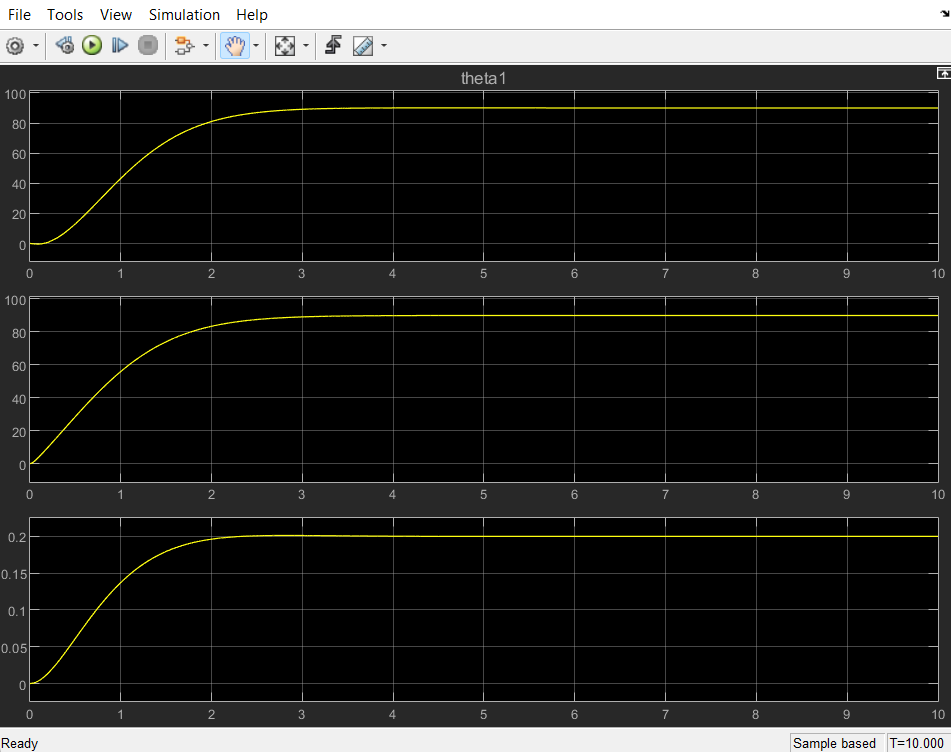
\includegraphics[width=0.8\textwidth]{resources/images/PID_res_m0.png}
    \caption{\centering{استجابة متحكم \LR{PID} بدون حمل ($m_L = 0 \text{ kg}$)}}
    \label{fig:pid_m0}
\end{figure}
  

\begin{figure}[H]
    \centering
    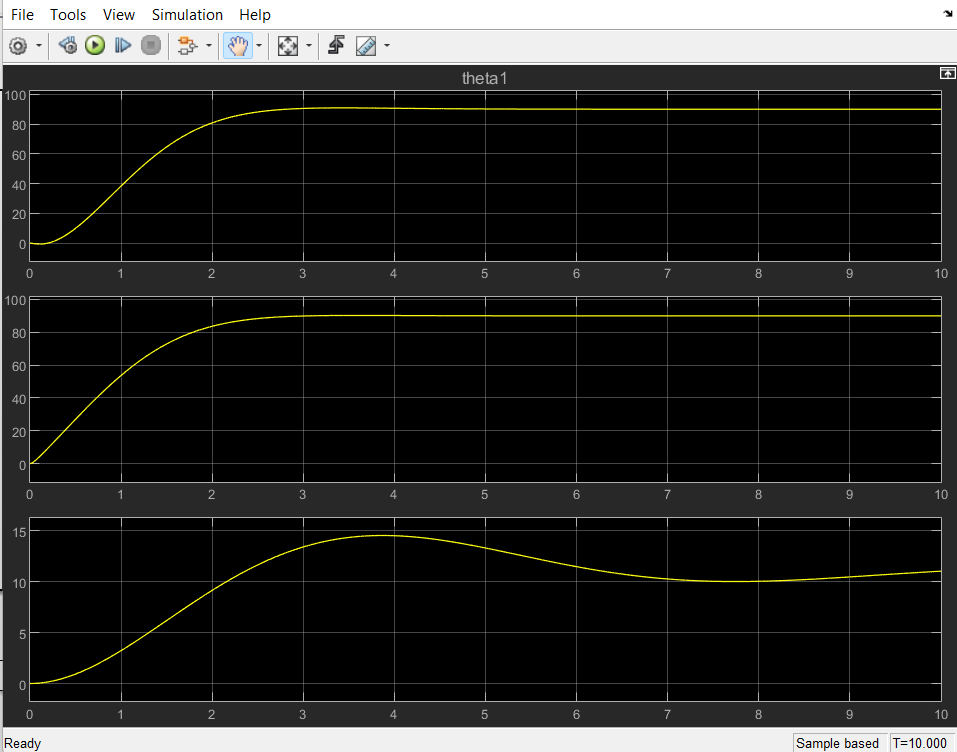
\includegraphics[width=0.8\textwidth]{resources/images/PID_res_m10.png}
    \caption{\centering{استجابة متحكم \LR{PID} عند إضافة حمل ($m_L = 10 \text{ kg}$)}}
    \label{fig:pid_m10}
\end{figure}

يُلاحظ من الشكل (\ref{fig:pid_m0}) أن المتحكم في حالة اللاحمل ($m_L = 0$) قادر على توجيه المفاصل نحو القيم المرجعية بدقة واستقرار تام وبدون خطأ حالة مستقرة. 

في المقابل، عند إضافة حمل كتلته ($10 \text{ kg}$) كما في الشكل (\ref{fig:pid_m10})، يتدهور أداء المتحكم الكلاسيكي بشكل حاد. يظهر هذا الانهيار بوضوح شديد في المفصل الانسحابي ($d_3$)، حيث ينحرف المسار الفعلي بشكل كارثي مبتعداً عن القيمة المرجعية ($0.2$) ليصل إلى قيم تفوق ($14$). يعود هذا الفشل إلى عجز أرباح الـ (\LR{PID}) الثابتة عن توليد إشارة تحكم كافية لتعويض الزيادة الضخمة في قوى الجاذبية وعزوم القصور الذاتي الناتجة عن الحمل الجديد، مما يثبت افتقار هذه الخوارزمية للمتانة (\LR{Robustness}) المطلوبة في التطبيقات الصناعية متغيرة الأوزان.
\section{التحكم بالانزلاق (\LR{Sliding Mode Control - SMC})}
\label{sec:smc_control}

\subsection*{1. مبدأ الخوارزمية}
تُصنف خوارزمية التحكم بالانزلاق (\LR{SMC}) كواحدة من أقوى استراتيجيات التحكم اللاخطي المتين (\LR{Robust Control}). تعتمد الفكرة الأساسية على إجبار مسار النظام الديناميكي للوصول إلى سطح رياضي مصمم مسبقاً يُدعى "سطح الانزلاق" (\LR{Sliding Surface})، ثم إبقائه مقيداً على هذا السطح. يوفر هذا الأسلوب مناعة عالية جداً ضد التغيرات المعلمية (مثل تغير كتلة الحمل) والاضطرابات الخارجية.

\subsection*{2. الشكل العام لقانون التحكم}
يتكون قانون التحكم بالانزلاق من مركبين أساسيين:
\begin{equation}
u(t) = u_{eq}(t) + u_{sw}(t)
\end{equation}
حيث:
\begin{itemize}
    \item $u_{eq}$: قانون التحكم المكافئ (\LR{Equivalent Control})، وظيفته إبقاء النظام على السطح بافتراض عدم وجود اضطرابات (يعتمد على النموذج الاسمي).
    \item $u_{sw}$: قانون التبديل (\LR{Switching Control})، وظيفته التغلب على الشكوك ودفع النظام نحو السطح في حال انحرافه عنه.
\end{itemize}

\subsection*{3. تهيئة النموذج وتعريف الأخطاء}
باستخدام نفس تعريفات الخطأ الموضعي $e = q_{ref} - q$ وخطأ السرعة $\dot{e} = \dot{q}_{ref} - \dot{q}$، يتم تعريف شعاع سطح الانزلاق $S$ بأبعاد $3 \times 1$ لمفاصل الروبوت بالمعادلة:
\begin{equation}
S = \dot{e} + \Lambda e
\end{equation}
حيث $\Lambda$ مصفوفة قطرية موجبة تماماً تحدد ميل سطح الانزلاق وسرعة تقارب الخطأ نحو الصفر. 
بأخذ المشتق الزمني لسطح الانزلاق نحصل على:
\begin{equation}
\dot{S} = \ddot{e} + \Lambda \dot{e} = \ddot{q}_{ref} - \ddot{q} + \Lambda \dot{e}
\end{equation}

\subsection*{4. تطبيق الخوارزمية على النموذج}
بالاعتماد على النموذج الديناميكي الشامل للروبوت المستنتج في الفصل السابق: $\ddot{q} = \bar{M}^{-1} [A u - R \dot{q} - D]$، نقوم بتعويض $\ddot{q}$ في معادلة $\dot{S}$:
\begin{equation}
\dot{S} = \ddot{q}_{ref} - \bar{M}^{-1} [A u - R \dot{q} - D] + \Lambda \dot{e}
\end{equation}
لإيجاد التحكم المكافئ $u_{eq}$، نضع $\dot{S} = 0$، فنحصل على:
\begin{equation}
u_{eq} = A^{-1} \left[ \bar{M} (\ddot{q}_{ref} + \Lambda \dot{e}) + R \dot{q} + D \right]
\end{equation}
لضمان شرط الوصول لسطح الانزلاق (\LR{Reachability Condition}) في ظل وجود تغير في الكتلة، نضيف حد التبديل باختيار $u_{sw} = A^{-1} \bar{M} K \text{sgn}(S)$، حيث $K$ مصفوفة أرباح التبديل القطرية. ليصبح قانون التحكم النهائي المطبق على المحركات:
\begin{equation}
u_{SMC} = A^{-1} \left[ \bar{M} (\ddot{q}_{ref} + \Lambda \dot{e}) + R \dot{q} + D + K \text{sgn}(S) \right]
\end{equation}

\subsection{5. استجابة النظام عند قيم مختلفة للحمل ($m_L$)}
تم اختبار خوارزمية (\LR{SMC}) على نفس المسارات المرجعية السابقة ($\theta_{1ref} = \theta_{2ref} = 90^\circ$ و $d_{3ref} = 0.2 \text{ m}$). توضح الأشكال التالية متانة المتحكم عند تغير الحمل:


 \begin{figure}[H]
     \centering
     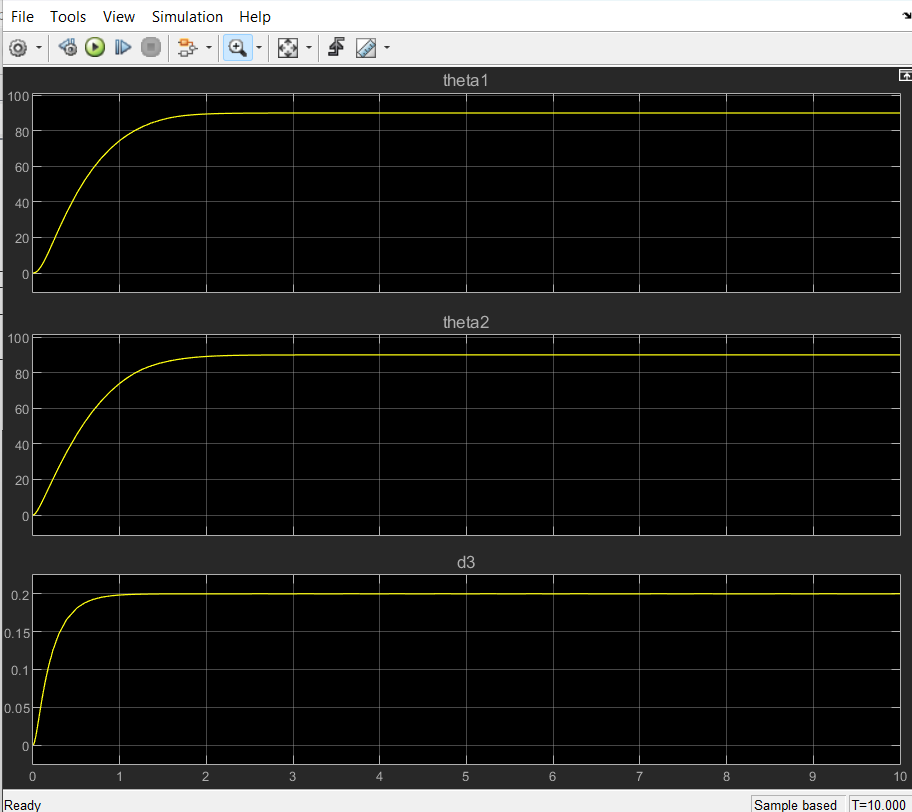
\includegraphics[width=0.8\textwidth]{resources/images/SMC_res_m0.png}
     \caption{\centering{استجابة متحكم \LR{SMC} بدون حمل ($m_L = 0 \text{ kg}$)}}
     \label{fig:smc_m0}
 \end{figure}

 \begin{figure}[H]
     \centering
     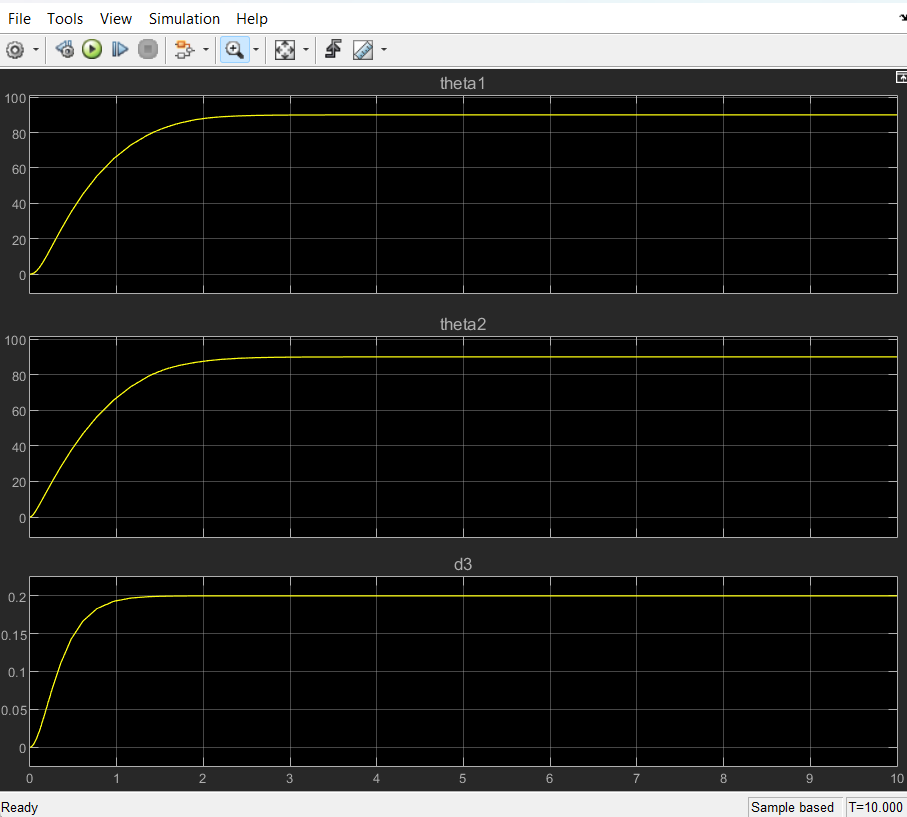
\includegraphics[width=0.8\textwidth]{resources/images/SMC_res_m10.png}
     \caption{\centering{استجابة متحكم \LR{SMC} عند إضافة حمل ($m_L = 10 \text{ kg}$)}}
     \label{fig:smc_m10}
 \end{figure}

على عكس الانهيار الذي حدث في خوارزمية (\LR{PID})، يُلاحظ من المنحنيات أن متحكم (\LR{SMC}) حافظ على دقة تتبع عالية للمسار المرجعي واستقرار ممتاز في المفصل الانسحابي حتى عند إضافة الحمل الأقصى ($10 kg$)، حيث استغرق النظام زمناً يقارب ($1 sec$) ليصل إلى حالة الاستقرار التام. يعود هذا الأداء المتين إلى تأثير حد التبديل اللاخطي الذي يجبر النظام على البقاء ضمن سطح الانزلاق المنيع ضد الاضطرابات الخارجية وتغيرات القصور الذاتي.
\section{التحكم التكيفي المعتمد على العزم المحسوب (\LR{Adaptive Computed Torque Control})}
\label{sec:actc_control}

\subsection*{1. مبدأ الخوارزمية}
تدمج هذه الخوارزمية بين تقنية الإلغاء الخطي للديناميكية (\LR{Feedback Linearization}) وبين آلية تكيفية مستمرة لتحديث معلمات النظام المجهولة (مثل كتلة الحمل وعزوم القصور الذاتي) في الزمن الفعلي. يتم استبدال الثوابت الفيزيائية المجهولة بمعلمات مُقَدَّرَة تتحدث قيمتها بناءً على خطأ التتبع، مما يوفر أداءً ناعماً ومستقراً دون الحاجة لإشارات التبديل القاسية.

\subsection*{2. الشكل العام لقانون التحكم ومبدأ الانحدار}
تعتمد الخوارزمية على خاصية خطية المعلمات (\LR{Linearity in Parameters})، حيث يمكن فصل النموذج الديناميكي إلى مصفوفة انحدار (\LR{Regressor} $Y$) تحوي المتغيرات الحركية المعروفة، وشعاع معلمات ($\Theta$) يحوي الثوابت المجهولة. 

لتطبيق الخوارزمية بشكل عملي ومستقل لكل مفصل، يُكتب قانون التحكم التكيفي للمفصل $(i)$ بالصيغة القياسية التالية:
\begin{equation}
\tau_i = \hat{\theta}_i^T Y_i - K_{s,i} s_i
\label{eq:adaptive_general_i}
\end{equation}
حيث $\hat{\theta}_i$ هو شعاع المعلمات المُقَدَّرَة للمفصل، و $Y_i$ شعاع الانحدار الخاص به، و $s_i$ هو سطح الانزلاق، و $K_{s,i}$ ربح تحكم موجب لضمان تقارب الخطأ.

\subsection*{3. تفكيك النموذج وتعريف المعلمات المُقَدَّرَة}
بتفصيل المعادلة (\ref{eq:adaptive_general_i}) بناءً على القوى الفيزيائية المؤثرة على المفصل (عطالة، احتكاك، جاذبية)، يأخذ قانون التحكم شكله التفصيلي المطبق على المحركات كما يلي:
\begin{equation}
\tau_i = \hat{\theta}_{M,i} (M_e(q)\ddot{q}_r)_i + \hat{\theta}_{V,i} (K_v \dot{q})_i + \hat{\theta}_{G,i} G_i(q) + \hat{\theta}_{0,i} - K_{s,i} s_i
\label{eq:adaptive_detailed_i}
\end{equation}

حيث تم تخصيص معامل مُقَدَّر منفصل لكل مركب ديناميكي:
\begin{itemize}
    \item $\hat{\theta}_{M,i}$: المُعامل التكيفي المُقَدَّر لتعويض تغيرات عزم القصور الذاتي الكلي (والذي يتأثر بشدة بتغير كتلة الحمل $m_L$).
    \item $\hat{\theta}_{V,i}$: المُعامل المُقَدَّر لتعويض قوى الاحتكاك اللزج والقوى المرتبطة بالسرعة.
    \item $\hat{\theta}_{G,i}$: المُعامل المُقَدَّر لتعويض عزوم الجاذبية الأرضية.
    \item $\hat{\theta}_{0,i}$: المُعامل المُقَدَّر لتعويض الاحتكاك السكوني (\LR{Coulomb Friction}) والاضطرابات الثابتة المجهولة.
\end{itemize}

\subsection*{4. تعريف الأخطاء وقانون التحديث (\LR{Adaptation Law})}
يتم تعريف سطح الانزلاق للمفصل $(i)$ بالاعتماد على خطأ التتبع الموضعي $e_i = q_i - q_{ref,i}$ كالتالي:
\begin{equation}
s_i = \dot{e}_i + \lambda_i e_i
\end{equation}
حيث $\lambda_i$ ثابت إيجابي يحدد ميل السطح. ولتحديث المعلمات المُقَدَّرَة $\hat{\theta}_i$ لحظياً وبشكل يضمن استقرار النظام وفق نظرية ليابونوف، يتم تطبيق قانون التحديث التفاضلي المدعوم بتعديل سيغما (\LR{$\sigma$-modification}) لمنع انحراف القيم:
\begin{equation}
\dot{\hat{\theta}}_i = \Gamma_i Y_i^T s_i - \Gamma_i \sigma_i \hat{\theta}_i
\end{equation}
حيث $\Gamma_i$ مصفوفة أرباح التعلم اللحظي، و $\sigma_i$ عامل تخميد إيجابي صغير.
\subsection*{5. استجابة النظام عند قيم مختلفة للحمل ($m_L$)}
تم اختبار خوارزمية (\LR{ACTC}) لمحاكاة تتبع المسارات المرجعية ($\theta_{1ref} = \theta_{2ref} = 90^\circ$ و $d_{3ref} = 0.2 \text{ m}$) مع تغيير ظروف التحميل للتحقق من قدرة الخوارزمية على التكيف الذاتي:


 \begin{figure}[H]
     \centering
     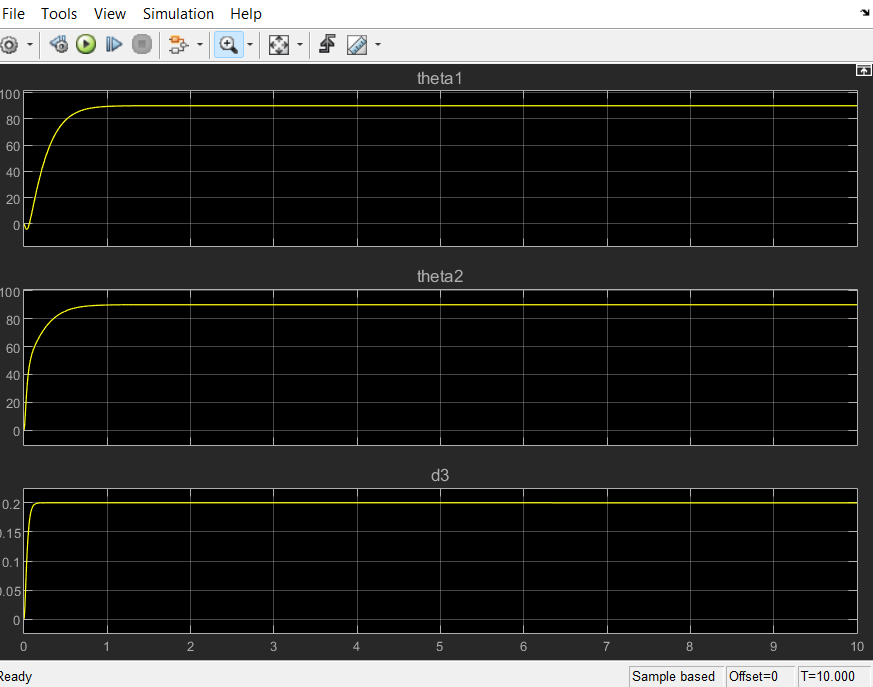
\includegraphics[width=0.8\textwidth]{resources/images/ACTC_res_m0.png}
     \caption{\centering{استجابة متحكم \LR{ACTC} وتتبع المسار بدون حمل ($m_L = 0 \text{ kg}$)}}
     \label{fig:actc_m0}
 \end{figure}

 \begin{figure}[H]
     \centering
     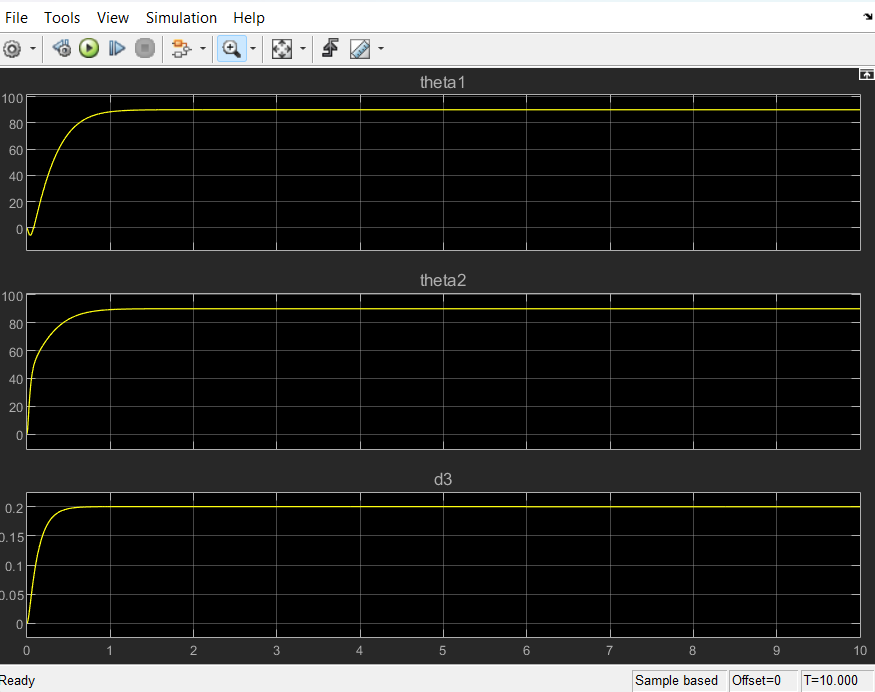
\includegraphics[width=0.8\textwidth]{resources/images/ACTC_res_m10.png}
     \caption{\centering{استجابة متحكم \LR{ACTC} وتحديث المعلمات لحظياً عند إضافة حمل ($m_L = 10 \text{ kg}$)}}
     \label{fig:actc_m10}
 \end{figure}

يُلاحظ من المنحنيات ظهور انحراف أولي سالب (\LR{Initial Undershoot}) لفترة وجيزة جداً في استجابة المفصل الأول ($\theta_1$) قبل انطلاقه نحو القيمة المرجعية. هذا الانحراف يعكس الطبيعة الفيزيائية الدقيقة للمحاكاة والتداخل الديناميكي (\LR{Dynamic Coupling}) بين المفاصل؛ فالتسارع الابتدائي العنيف للمفصل الثاني لتتبع المسار يولد عزم رد فعل يؤثر عكسياً على المفصل الأول، وسرعان ما تقوم خوارزمية (\LR{ACTC}) بتدارك هذا الاضطراب اللحظي وتصحيح المسار بقوة ونعومة.

بشكل عام، تظهر النتائج تفوقاً ديناميكياً وهندسياً واضحاً للمتحكم التكيفي. في حالة اللاحمل ($m_L = 0$)، استجاب النظام بسرعة فائقة محققاً زمن استقرار (\LR{Settling Time}) يقارب ($0.1 \text{ s}$). أما عند إضافة الحمل الأقصى المفاجئ ($10 \text{ kg}$)، فبدلاً من الانهيار كما في (\LR{PID}) أو استهلاك طاقة تبديل قاسية كما في (\LR{SMC})، قامت الآلية التكيفية بتقدير الزيادة اللحظية في القصور الذاتي وتحديث المعامل $\hat{\theta}_{M,3}$ داخلياً، ليتمكن النظام من استعادة استقراره التام خلال زمن قياسي لم يتجاوز ($0.5 \text{ s}$). نتج عن ذلك تتبع مسار عالي الدقة، وإشارات تحكم ناعمة خالية من ظاهرة الاهتزاز (\LR{Chattering})، مما يجعله الحل الأمثل صناعياً.
\section{مقارنة استراتيجيات التحكم واختيار الخوارزمية الأمثل}
\label{sec:control_comparison}

بعد التطبيق والتحليل المعمق لخوارزميات التحكم الثلاث (\LR{PID}، \LR{SMC}، و \LR{ACTC}) على النموذج الديناميكي الشامل لروبوت (\LR{SCARA})، واختبارها تحت ظروف تحميل متغيرة (من حالة اللاحمل إلى حمل أقصى $m_L = 10 \text{ kg}$)، يمكن تلخيص الفروقات الجوهرية بين هذه الاستراتيجيات من حيث الأداء الديناميكي، المتانة، والعبء الحسابي في الجدول التالي:
\begin{table}[H]
    \centering
    \caption{مقارنة هندسية بين استراتيجيات التحكم المطبقة على الروبوت}
    \label{tab:control_comparison}
    % إضافة تعليمات إيقاف المط (raggedright) والتوسيط (centering) للأعمدة
    \begin{tabular}{|>{\centering\arraybackslash}p{0.14\linewidth}|>{\raggedright\arraybackslash}p{0.21\linewidth}|>{\raggedright\arraybackslash}p{0.22\linewidth}|>{\raggedright\arraybackslash}p{0.21\linewidth}|>{\centering\arraybackslash}p{0.12\linewidth}|}
        \hline
        \textbf{الخوارزمية} & \textbf{دقة التتبع الموضعي} & \textbf{المتانة ضد تغيرات الحمل ($m_L$)} & \textbf{زمن الاستقرار} & \textbf{التعقيد الحسابي برمجياً} \\
        \hline
        \textbf{الكلاسيكي (\LR{PID})} & ممتازة في حالة اللاحمل، وضعيفة عند السرعات العالية. & منهارة (تأثر شديد بزيادة عزم القصور الذاتي للوصلة). & سريع في اللاحمل، وينهار (يفقد الاستقرار) عند إضافة الحمل. & بسيط جداً (لا يتطلب نموذج رياضي). \\
        \hline
        \textbf{الانزلاقي (\LR{SMC})} & عالية جداً. & ممتازة (مناعة تامة ضد الاضطرابات الخارجية). & \centering{جيد} & متوسط (يتطلب معرفة النموذج الاسمي). \\
        \hline
        \textbf{التكيفي (\LR{ACTC})} & عالية جداً. & ممتازة (تكيف ذاتي وتقدير لحظي ). & \centering{قياسي وسريع } & عالي (يتطلب تفكيك وحساب مصفوفة الانحدار $Y$). \\
        \hline
    \end{tabular}
\end{table}

\subsection*{القرار الهندسي: اعتماد خوارزمية (\LR{ACTC})}
بناءً على المعطيات التحليلية السابقة وطبيعة المهمة الصناعية لروبوت (\LR{SCARA}) المدروس (والتي تتمثل في نقل حمولات متغيرة الوزن بسرعات عالية)، \textbf{تم اختيار خوارزمية التحكم التكيفي المعتمد على العزم المحسوب (\LR{ACTC})} لتكون الاستراتيجية النهائية والمعتمدة في هذا المشروع. 

يأتي هذا الاختيار مبرراً بالنقاط والمزايا الهندسية التالية:
\begin{enumerate}
    \item \textbf{زمن استجابة قياسي:} أثبتت الخوارزمية قدرتها على استعادة استقرار النظام وتصفير خطأ التتبع خلال زمن قصير جداً ($0.5 \text{ s}$) حتى عند تعرض الروبوت  لصدمة تحميل ($10 \text{ kg}$)، مع امتصاص ذكي لعزوم التداخل الديناميكي بين المفاصل.
    \item \textbf{الاستغناء عن المعايرة اليدوية:} قدرة المتحكم التلقائية على تقدير الزيادة في القصور الذاتي وتحديث المعاملات المجهولة (مثل $\hat{\theta}_{M,3}$) لحظياً، مما يغني عن الحاجة لإعادة ضبط أرباح التحكم يدوياً عند كل تغيير في وزن القطعة المنقولة.
    \item \textbf{الحفاظ على العمر الافتراضي للمحركات:} على عكس متحكم (\LR{SMC}) الذي يضمن المتانة على حساب إرهاق المحركات بجهود تبديلية عالية التردد (\LR{Chattering})، توفر خوارزمية (\LR{ACTC}) إشارات تحكم ناعمة ومستمرة خالية من الاهتزازات، مما يقلل من التآكل الميكانيكي في المفاصل والارتفاع الحراري في ملفات المحركات.
\end{enumerate}

بهذا الاستنتاج، نكون قد أتممنا تصميم واختبار "العقل" البرمجي القادر على قيادة ذراع الروبوت بكفاءة صناعية عالية.
\chapter{الخاتمة والتوصيات}

\section{الخاتمة }


شكل هذا المشروع دراسة تحليلية شاملة للنمذجة الرياضية وتطوير استراتيجيات التحكم للمناورات الروبوتية، مطبقةً على ذراع روبوت من نوع (\LR{SCARA}). لقد انطلق مسار البحث من التوصيف الهندسي المجرد للفضاء التشغيلي عبر استنتاج معادلات الحركة المباشرة (\LR{Forward Kinematics})، وصولاً إلى بناء نموذج ديناميكي متكامل باستخدام صياغة لاغرانج-أويلر (\LR{Euler-Lagrange}). تميز هذا النموذج بدقته الفيزيائية من خلال دمج ديناميكية المحركات الكهربائية (\LR{Actuator Dynamics}) وأخذ التغيرات اللحظية في موقع مركز الثقل وعزوم القصور الذاتي للوصلة الثالثة بعين الاعتبار عند نقل الحمولات.

في شق التحكم، أثبتت الدراسة التحليلية وعمليات المحاكاة قصور خوارزميات التحكم الكلاسيكية المستقلة (\LR{PID}) عن تلبية متطلبات الأداء الصناعي عند تغير كتل التحميل، حيث أظهرت استجابة النظام انهياراً ملحوظاً في المفصل الانسحابي. لمعالجة هذه المعضلة، تم الانتقال إلى التحكم اللاخطي المتين عبر خوارزمية التحكم بالانزلاق (\LR{SMC})، والتي وفرت مناعة تامة ضد الاضطرابات، ولكن على حساب إجهاد المحركات بظاهرة الاهتزاز (\LR{Chattering}). 

توجت هذه الدراسة بتصميم واختبار خوارزمية التحكم التكيفي المعتمد على العزم المحسوب (\LR{ACTC}). أثبتت هذه الخوارزمية تفوقها الهندسي المطلق من خلال قدرتها على التكيف الذاتي، وتقدير الزيادة اللحظية في القصور الذاتي بشكل برمجي ذكي، مما أثمر عن تحقيق دقة تتبع مسار استثنائية، وزمن استقرار قياسي، وإشارات تحكم ناعمة تضمن إطالة العمر الافتراضي للمنظومة الكهروميكانيكية.

\section{التوصيات للعمل المستقبلي }

بناءً على النتائج المستخلصة من هذا البحث، وللارتقاء بأداء المنظومة الروبوتية نحو تطبيقات صناعية أكثر تعقيداً، نُدرج التوصيات الهندسية التالية للعمل المستقبلي:

\begin{enumerate}
    \item \textbf{التقدير الآلي والمسبق لكتلة الحمل ($m_L$):} 
    رغم كفاءة خوارزمية (\LR{ACTC}) في التكيف الرياضي مع القصور الذاتي المجهول، يُوصى بتزويد المؤثر النهائي للروبوت بحساسات قوة/عزم (\LR{Force/Torque Sensors})، أو تصميم مراقب حالة متقدم (\LR{State Observer}) لتقدير كتلة الحمل الديناميكية آلياً بمجرد التقاط القطعة. إدخال هذه القيمة المُقاسة مباشرةً إلى خوارزمية التحكم سيختصر زمن التكيف الابتدائي ويمنع أي انحراف أولي (\LR{Initial Undershoot}) أثناء التسارع المفاجئ.

    \item \textbf{توسيع النموذج الديناميكي للسرعات الفائقة:}
    في مهام النقل والتوضيع (\LR{Pick and Place}) التي تتطلب سرعات حركية فائقة جداً، يُوصى بإعادة دمج مصفوفة قوى كوريوليس والطرد المركزي $C(q, \dot{q})$ التي تم إهمالها في هذه الدراسة. سيؤدي دمج هذه القوى غير الخطية إلى زيادة التعقيد الحسابي، ولكنه سيرفع من دقة النموذج التنبؤي في ظروف التشغيل القاسية.
\end{enumerate}









%==================== المراجع ====================

\renewcommand{\bibname}{المراجع}
\addcontentsline{toc}{chapter}{المراجع}

\begin{thebibliography}{9}


\bibitem{craig2005}
\LR{Craig, J. J. (2005). \textit{Introduction to Robotics: Mechanics and Control} (3rd ed.). Pearson Prentice Hall.}


\bibitem{slotine1991}
\LR{Slotine, J. J. E., \& Li, W. (1991). \textit{Applied Nonlinear Control}. Prentice Hall.}

\end{thebibliography}


\end{document}